\documentclass{article}
\usepackage[UTF8]{ctex}
\usepackage{geometry}
\usepackage{natbib}
\geometry{left=3.18cm,right=3.18cm,top=2.54cm,bottom=2.54cm}
\usepackage{graphicx}
\pagestyle{plain}	
\usepackage{setspace}
\usepackage{caption2}
\usepackage{datetime} %日期
\renewcommand{\today}{\number\year 年 \number\month 月 \number\day 日}
\renewcommand{\captionlabelfont}{\small}
\renewcommand{\captionfont}{\small}
\begin{document}

\begin{figure}
    \centering
    
\includegraphics[width=8cm]{upc.png}

    \label{figupc}
\end{figure}

	\begin{center}
		\quad \\
		\quad \\
		\heiti \fontsize{45}{17} \quad \quad \quad 
		\vskip 1.5cm
		\heiti \zihao{2} 《计算科学导论》课程总结报告
	\end{center}
	\vskip 2.0cm
		
	\begin{quotation}
% 	\begin{center}
		\doublespacing
		
        \zihao{4}\par\setlength\parindent{7em}
		\quad 

		学生姓名:\underline{\qquad  孙萃 \qquad \qquad}

		学\hspace{0.61cm} 号:\underline{\qquad 2007010219\qquad}
		
		专业班级:\underline{\qquad 计科2002 \qquad  }
		
        学\hspace{0.61cm} 院:\underline{计算机科学与技术学院}
% 	\end{center}
		\vskip 2cm
		\centering
		\begin{table}[h]
            \centering 
            \zihao{4}
            \begin{tabular}{|c|c|c|c|c|c|c|}
            % 这里的rl 与表格对应可以看到,姓名是r,右对齐的;学号是l,左对齐的;若想居中,使用c关键字。
                \hline
                课程认识 & 问题思 考 & 格式规范  & IT工具  & Latex附加  & 总分 & 评阅教师 \\
                30\% & 30\% & 20\% & 20\% & 10\% &  &  \\
                \hline
                 & & & & & &\\
                & & & & & &\\
                \hline
            \end{tabular}
        \end{table}
		\vskip 2cm
		\today
	\end{quotation}

\thispagestyle{empty}
\newpage
\setcounter{page}{1}
% 在这之前是封面,在这之后是正文
\section{引言}
计算科学导论这门课程,是面对大学计算机科学系一年级学生的,作为导引性课程的教材。本课程从如何成长为一个优秀的专业技术人才,从更一般的认识层面上掌握如何学习一门新的学科专业知识的方式方法,解决如何认识计算机科学与技术,如何学习计算机科学与技术的问题。\par
导论的目的在于从科学哲学的角度用高级科普的形式为初学者提供一个了解 和学习计算机科学与技术领域的专门的,具体的,系统的专业技术知识,特别要 注意避免焦躁情绪的产生。而且导论并不系统地阐述科学哲学与学科方法论的内容,而是将科学哲学的观点与学科方法论中大量成熟的内容融入到各章节之中,自始至终贯穿在各个章节的字里行间中。导论中很少涉及具体的,系统的专业知 识特别是操作使用计算机的技术知识,不必感到困惑,因为导论仅是为我们以后 学习基础课程和后续计算机科学与技术的一个导引,一些名词和术语,以后会在一些具体的分支学科课程中学到,其中的许多观点和思想方法,对整个大学生涯是大有裨益的。\par
正如孙老师所说,计算机专业是宇宙第一专业,我也很荣幸在中国石油大学(华东)就读计算机科学与技术专业。并且很幸运的学习了由博学多才,科学严谨的孙老师教授的计算导论这门课程,通过幽默而严谨的话语传授知识,对此我有所感悟,接下来就据此撰写课程报告。\par
\section{对计算科学导论这门课程的认识、体会}
导论是针对计算机科学初学者而开设的,它在一个初学者对整个学科还缺乏深入,全面了解的情况下,从科学哲学的角度对计算机科学与技术的定义,范畴,特点,基本问题,发展主线,学科分类,知识组织结构,学科发展的特点和内在 规律以及从事学科工作的基本工作流程建立起一种基本的,科学概貌性的认识,对如何使自己富有创新意识,逐步成长为创新人才建立起一种基本的,正确的科 学认识。它并不要求初学者广泛借阅图书资料,因为初学者并不具备同时掌握几体系的能力与知识基础,并且很少涉及具体的,系统的专业知识,特别是操作 使用计算机的的技术知识,它仅是为初学者学习基础课程和后续计算机科学与技术课程的一个导引。\par
例如导论从计算科学一词的来历开始介绍,依次介绍了科学哲学,科学认识论,科学方法论,学科方法论。二进制,通用数学计算机系统结构与工作原理,数学逻辑与集成电路,机器指令与汇编语言,算法,过程与程序,高级语言与程序设计,程序设计方法与技术,系统软件与应用软件,计算机图形学,图像处理与模式识别,逻辑与人工智能,计算机组织与体系组织,并行计算机系统,通道与并行计算,计算机网络与通信,高性能计算以及学科的基本问题,计算学科的学科形态与核心形态与核心概念,计算科学的典型方法与典型实例,学科基本工作流程方式及学科意义,计算科学学科特点,发展规律,趋势及其社会影响。计算科学组织结构 及其演变,计算机产业发展前景以及如何学习计算科学与健康成长。\par
这些对计算学科全方位的介绍,以及各章节中贯穿的科学哲学和学科方法论,虽然浅尝辄止,但让初学者甘之如饴,建立起对本学科认识的基本框架,激发兴趣。任何一门学科学科或专业,都含有丰富的人文内容和特质,都可以进行人文教育,使学生在学习中感受到美的熏陶与生命力量的提升,在计算学科导论的教学过程中,以一种什么样的意义来揭示该学科,就帮助学生设置一个学习的方向。方向不同,学生在从事学习过程中进行的心理活动不同,学习的结果也不同。对知识,学生会记忆性地学,对技能,学生会模仿性地学,对能力方面,学生会思 维地学,对伦理方面,学生会体验地学。无论如何,教学过程中的引导作用是非 常明显也是极其重要的。并且相信几乎占据导论"半壁江山"的学科意义,内容,方法,健康成长是任意一本专业书都不会出现的。也就是说,本书是为了培养高 素质的计算机科学与技术专业人才的一个导引。在通识教育观下,引导初学者具 备高素质人才的条件: \par
(1)具有高尚的品德和良好的人文素养。\par
(2)具有坚实的专业基础和深厚的专业功底。\par
(3)具有创新意识,具有科学的思想方法。\par
\subsection{图灵机}
图灵机的等价机器:继续上节课没讲完的内容,我知道了,除了图灵机以外,人们还发明了很多其它的计算模型。包括:寄存器机、递归函数、λ演算、生命游戏、马尔可夫算法。\par

感悟:根据图灵机的工作原理,可想图灵机在日常生活中的应用之广泛,特别是将图灵机应用于人工智能,将会取代不少劳动力,另一方面,假设在图灵机的基础上设定更为复杂的状态,那么对AI机器人将会是史诗级的突破。
\subsection{迷宫}
这个题目和数据结构—图有关\par
迷宫的随机生成和路径搜索主要和图的遍历有关,一般来说图的遍历主要有两种方式:1、深度优先遍历(DFS)2、广度优先遍历(BFS)
两种遍历方式都很好理解,就说说深度优先遍历:
\par
深度优先遍历,顾名思义,就是尽可能往深处遍历,访问到一个节点时,搜索这个节点没有被访问过的相邻节点,选择一个继续做同样的操作,直到没有邻节点为止再回溯到上一个访问的节点,并选择另外的邻节点。
\par
可以这样描述深度遍历:

(1)访问顶点v;\par

(2)从v的未被访问的邻接点中选取一个顶点w,重复第一步,如果v没有未访问的邻接点,回溯至上一顶点\par

(3)重复上述两步,直至图中所有和v有路径相通的顶点都被访问到。

至于迷宫的路径搜索,那就完全是图的深度遍历了,大概过程如下。\par

(1)从迷宫起点节点V开始访问\par

(2)访问这个节点V,标记为可行的路径;\par

(3)从v的未被访问的非"墙"邻接点中选取一个顶点w,重复第二步。如果v没有未访问的非"墙"邻接点,把这个节点的可行路径标记移除,回溯至上一节点;\par

(4)重复上述第(2)、(3)步,直至遍历到迷宫的出口节点。\par

\subsection{大数据可视化}

我阅读了图书《基于WebGIS的新冠肺炎疫情可视化系统研发》\citep{基于WebGIS的新冠肺炎疫情可视化系统研发2020},引发了我对可视化系统的兴趣,于是阅读了期刊论文《》大数据平台的测震数据流实时可视化系统设计与实现》\citep{大数据平台的测震数据流实时可视化系统设计与实现}。我又阅读了《基于大数据可视化技术的信息系统AC审计》\citep{基于大数据可视化技术的信息系统AC审计}。\par


\section{进一步的思考}

\begin{itemize}
   \item 课题:大数据可视化\par
    a) 概念\par
     大数据可视化是将大量的异构系统数据进行采集,整合及利用大数据分析能力和计算机视觉技术,结合关联分析、空间分析和多维分析等多种分析手段,挖掘对应数据业务算法模型,最终将分析结果通过可视化的界面进行展示,为高层领导提供业务决策依据,引导决策者做出有效的决策,实现大数据落地的业务场景,体现数据价值,全面提高决策层数据可视化、信息化水平。\par
    b) 相关基本概念\par
    ①数据空间:是由n维属性和m个元素组成的数据集所构成的多维信息空间;\par
    ②数据开发:是指利用一定的算法和工具对数据进行定量的推演和计算;\par
    ③数据分析:指对多维数据进行切片、块、旋转等动作剖析数据,从而能多角度多侧面观察数据;\par   
    c)方向\par
      (1)宏观态度可视化:态势可视化是在特定环境中对随时间推移而不断动作并变化的目标实体进行觉察、认知、理解,最终展示整体态势。此类大数据可视化应用通过建立复杂的仿真环境,通过大量数据多维度的积累,可以直观、灵活、逼真地展示宏观态势,从而让非专业人士很快掌握某一领域的整体态势、特征。\par
      ○	案例一:全球航班运行可视化系统,通过将某一时段全球运行航班的飞行数据进行可视化展现,大众可以很清晰的得以了解全球航班整体分布与运行态势情况。\par
      ○	案例二:卫星分布运行可视化通过将宇宙空间内所有卫星的运行数据进行可视化展示,大众可以一目了然宇宙空间的卫星态势。\par
      (2)设备仿真运行可视化:通过图像、三维动画以及计算机程控技术与实体模型相融合,实现对设备的可视化表达,使管理者对其所管理的设备有形象具体的概念,对设备所处的位置、外形及所有参数一目了然,会大大减少管理者的劳动强度,提高管理效率和管理水平。\par
      ○	案例一:军工领域战场设备可视化在战场环境中对作战区域内随时间推移而不断动作并变化的作战实体进行可视化展示。了解敌我双方的兵力部署,进而指挥部署我方的兵力应对和决策。\par
      ○	案例二:卫星运行可视化卫星可视化可以了解大范围卫星态势,并对卫星的轨道、在轨姿态、卫星所执行的任务可视化呈现,主要包括:飞行、变轨、侦查,扫描,数据传输等等。除此之外,对卫星回传的数据,卫星自身的状态,也有针对性的可视化分析和监测。\par
      (3)数据统计分析可视化:此领域是目前媒体大众提及最多的应用,可用于商业智能、政府决策、公众服务、市场营销等领域。\par
      ○商业智能可视化通过采集相关数据,进行加工并从中提取能够创造商业价值的信息,面向企业、政府战略并服务于管理层、业务层,指导经营决策。商业智能可视化负责直接与决策者进行交互,是一个实现了数据的浏览和分析等操作的可视化、交互式的应用。\par
    d)可视化图形的选择与构建\par
    设计可视化作品时应该充分考虑,比如:\par
    •	避免使用面积图作为对比\par
    •	在做对比类图形时,当差异不明显时需要考虑采用非线性的视觉元素\par
    •	选用多种颜色作为视觉编码时,差异应该足够大\par
    
    	(1)常见的21种常见大数据可视化图表(下面是各种图形的例子和不同情况的选择) :\par
    		1)柱状图:用垂直或水平的柱子表示不同分类数据的数值大小
    		虽然能展示数据的变化趋势,但这并非它的强项\par
    		\begin{figure}[h!]
    			\centering
    			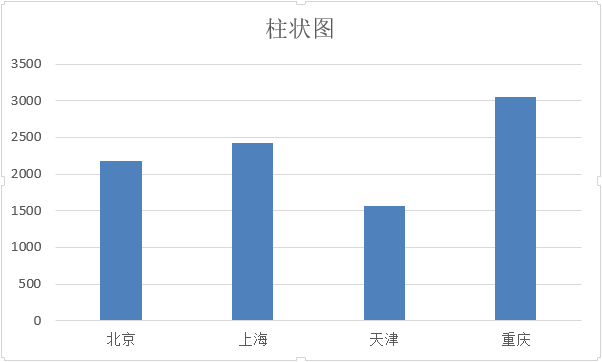
\includegraphics[scale=0.7]{zhuzhuangtu}
    			\caption{The 柱状图}
    			\label{fig:zhuzhuangtu}
    		\end{figure}
    		2)堆积柱状图:适用于包含若干个小分类的分组数据的可视化
    		用于比较同一分组内不同分类的数据,或者各组的总量
    		无法比较不同分组内相同分类的数据
    		同一组数据分类过多会降低图表易读性\par
    		\begin{figure}[h!]
    			\centering
    			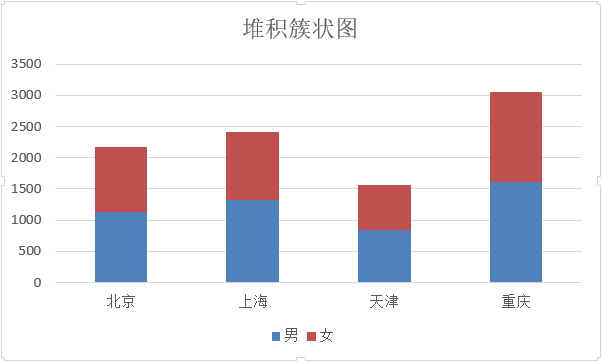
\includegraphics[scale=0.7]{duiji}
    			\caption{The 堆积柱状图}
    			\label{fig:duiji}
    		\end{figure}
    	.\par.\par.\par.\par.\par
    		3)分组柱状图:适用于包含了相同分类的多组数据的比较
    		可以比较同一分组内不同分类的数据,或不同分组内相同分类的数据
    		无法对比各分组的总量\par
    		\begin{figure}[h!]
    			\centering
    			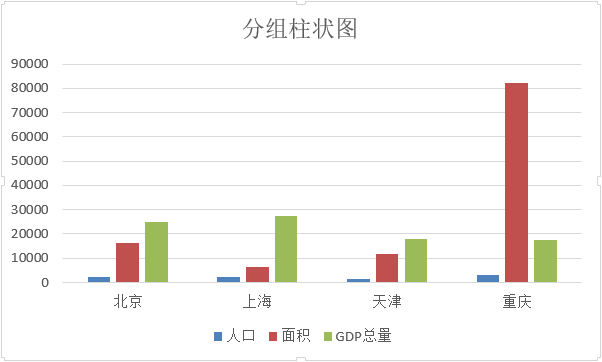
\includegraphics[scale=0.7]{fenzu}
    			\caption{The 分组柱状图}
    			\label{fig:fenzu}
    		\end{figure}
    		4)正负条形图:使用正反向柱子表示数据的正负数值
    		适用于有相反含义的数据(例如不同国家的男性与女性的人口数量)
    		注意的是分界线需为0点\par
    		\begin{figure}[h!]
    			\centering
    			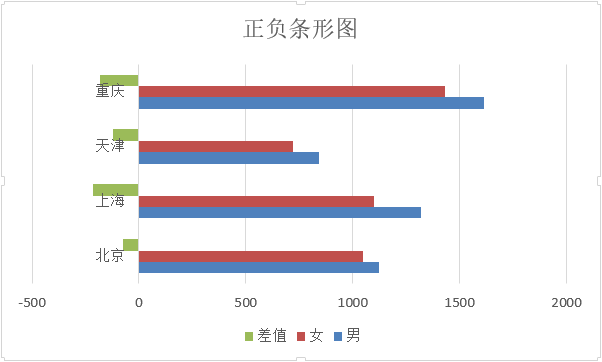
\includegraphics[scale=0.7]{zhengfu}
    			\caption{The 正负条形图}
    			\label{fig:zhengfu}
    		\end{figure}
    		5)组成瀑布图:用于展示数据的组成,或者增减变化过程
    		注意相邻浮动列的首尾要在同一水平线上\par
    	    \begin{figure}[h!]
    		\centering
    		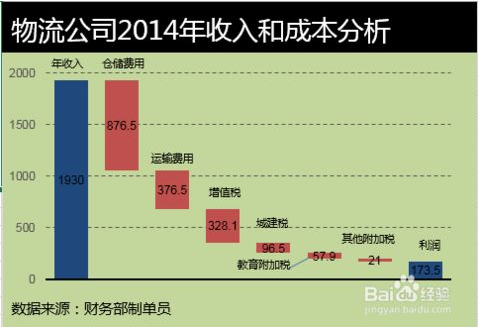
\includegraphics[scale=0.5]{zucheng}
    		\caption{The 组成瀑布图}
    		\label{fig:zucheng}
    		\end{figure}
    		6)折线对比图:适用于展示数据的连续变化趋势
    		注意自变量要有顺序关系(如时间)
    		注意因变量单位数值对于折线起伏变化的影响
    		折线过多会降低图表的易读性\par
    		\begin{figure}[h!]
    		\centering
    		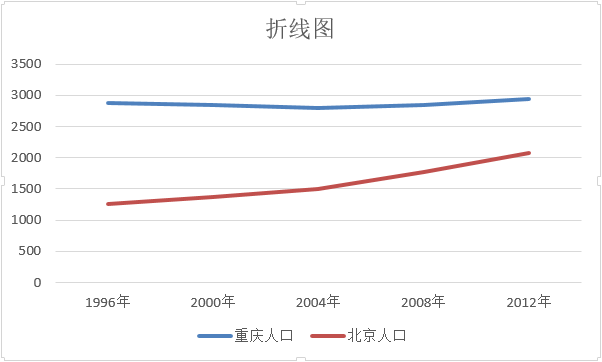
\includegraphics[scale=0.7]{zhexian}
    		\caption{The 折线对比图}
    		\label{fig:zhuzhuangtu}
    		\end{figure}
    		7)层叠面积图:用颜色填充折线与坐标轴之间的区域,以强调数据的变化趋势
    		注意颜色部分,要是用透明度来区分不同分类数据\par  
    		\begin{figure}[h!]
    		\centering
    		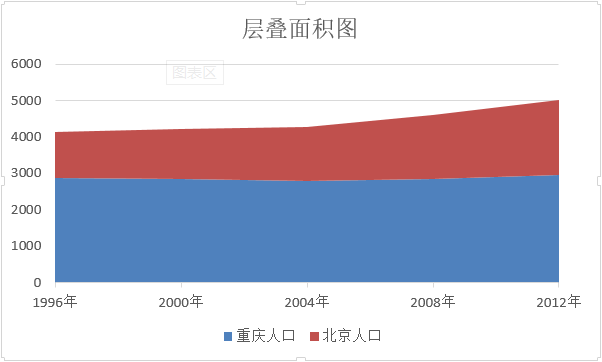
\includegraphics[scale=0.7]{cengdie}
    		\caption{The 层叠面积图}
    		\label{fig:cengdie}
    		\end{figure}
    		8)河流图:面积图的变形
    		展示不同类别的数据随时间变化的情况
    		注意数据可视化是围绕一个变化的中心基线而不是自变量轴\par
    		\begin{figure}[h!]
    			\centering
    			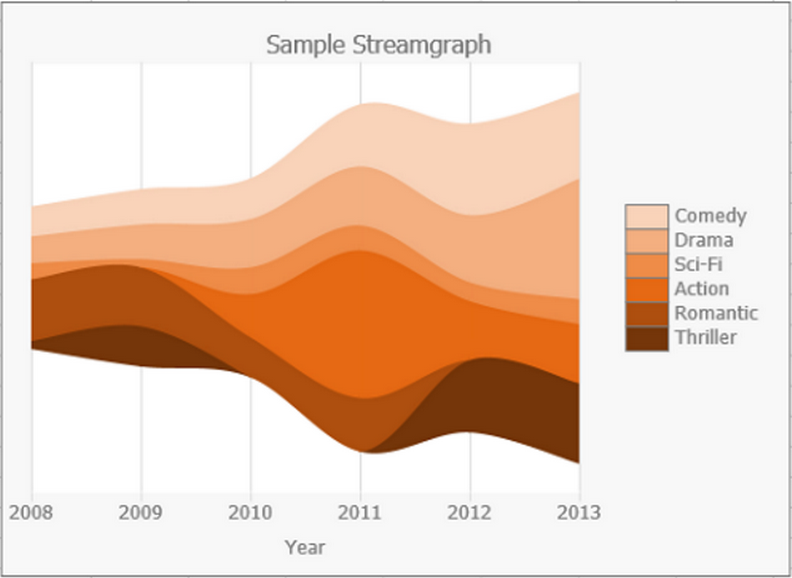
\includegraphics[scale=0.3]{heliu}
    			\caption{The 河流图}
    			\label{fig:heliu}
    		\end{figure}
    		.\par
    		9)基础饼图:通过扇形的角度大小展示各数据在整体种的占比大小
    		分类过多时,占比晓得分类数据会难以辨别
    		在展示区别不大的数据时,饼图的可视化效果会下降\par
    		\begin{figure}[h!]
    			\centering
    			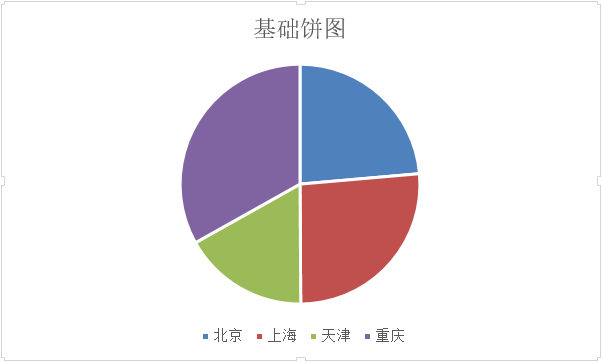
\includegraphics[scale=0.5]{bingtu}
    			\caption{The 基础饼图}
    			\label{fig:bingtu}
    		\end{figure}
    		10)环图:属于中心挖空的饼图
    		通过环块的角度大小展示各数据在整体中的占比大小\par
    		\begin{figure}[h!]
    			\centering
    			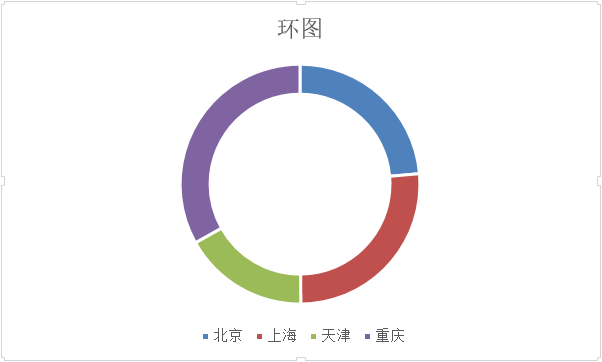
\includegraphics[scale=0.7]{huan}
    			\caption{The 环图}
    			\label{fig:huantu}
    		\end{figure}
    	
    		11)双层环图:属于中心挖空的饼图
    		双环之间有一层包含关系
    		适合展示有一层包含关系的数据占比情况
    		\par
    		\begin{figure}[h!]
    			\centering
    			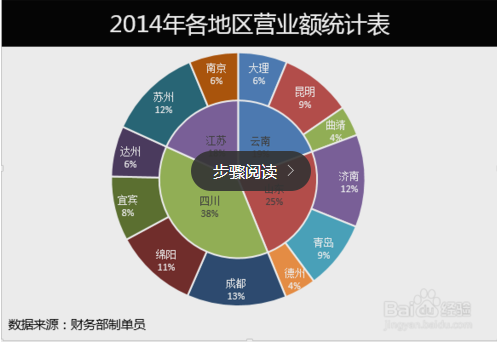
\includegraphics[scale=0.7]{shaung}
    			\caption{The 双层环图}
    			\label{fig:shaung}
    		\end{figure}
    		.\par.\par
    		12)南丁格尔玫瑰图:擅长凸显数据之间的差异,适用于比较大小相近的数值
    		不适合分类过少的数据(例如一个国家出生和死亡人数)
    		不适合数值相差过大的数据(例如世界各国人口数)\par
    		\begin{figure}[h!]
    			\centering
    			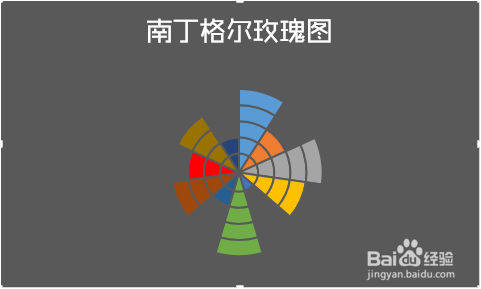
\includegraphics[scale=0.7]{nan}
    			\caption{The 南丁格尔玫瑰图}
    			\label{fig:nan}
    		\end{figure}
    		13)旭日图:饼图的变形,适用于展示多层级的数据的占比情况
    		通过环块的角度大小展示各数据在同环数据中的占比大小
    		相邻的两层数据通常有包含关系,越往外层,分类越细越具体
    		在数据量很大的是,要借助交互功能才能保持图表的易读性\par
    		\begin{figure}[h!]
    			\centering
    			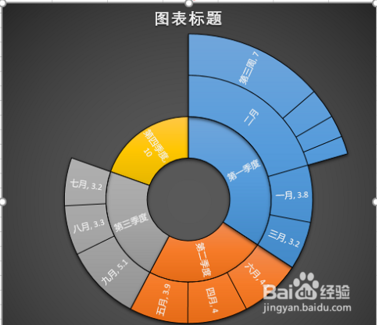
\includegraphics[scale=0.7]{xu}
    			\caption{The 旭日图}
    			\label{fig:xu}
    		\end{figure}
    
    		14)雷达图:坐标轴始于统一圆心径向排列
    		同一个分类数据的各项数值点围成一个多边形
    		擅长展示综合性能和突出异常数据
    		不适合变量或分类过多的数据\par
    		\begin{figure}[h!]
    			\centering
    			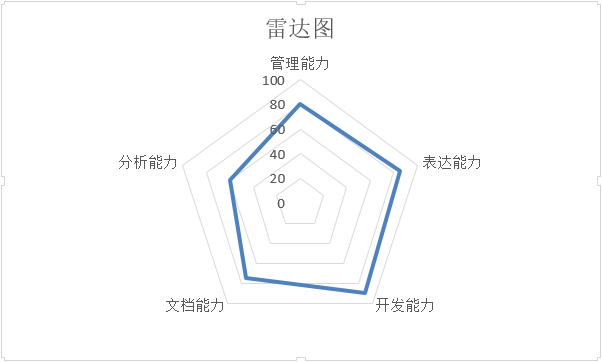
\includegraphics[scale=0.6]{leida}
    			\caption{The 雷达图}
    			\label{fig:leida}
    		\end{figure}
    		15)漏斗图:适用于具有逻辑顺序的分类数据的对比(例如看到问卷的人数—进入问卷填写页面的人数—完成问卷的人数—转发问卷的人数)
    		每个梯形的下底长度则代表该分类数据的数值大小\par
    		\begin{figure}[h!]
    			\centering
    			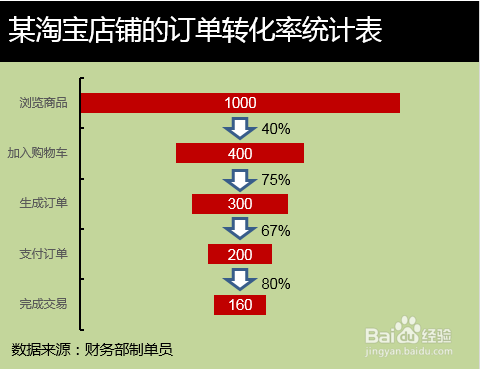
\includegraphics[scale=0.7]{loudou}
    			\caption{The 漏斗图}
    			\label{fig:loudou}
    		\end{figure}
    		16)散点图:通过点的位置展示数据的大小
    		通过点的分布观察不同分类数据的相关关系
    		分类数据过多会使点的数量过多,降低图表的易读性\par
    		\begin{figure}[h!]
    			\centering
    			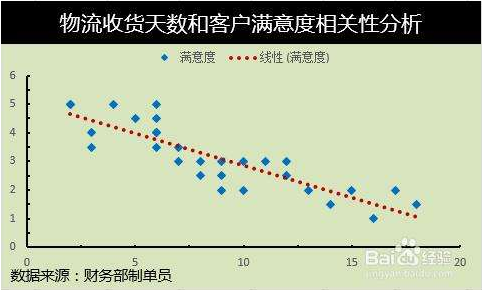
\includegraphics[scale=0.7]{san}
    			\caption{The 散点图}
    			\label{fig:sandian}
    		\end{figure}
    		17)立体气泡图:气泡图是基于散点图的多变量数据可视化形式
    		气泡的面积大小和颜色均可以表示数值
    		气泡过多会让气泡难以区分\par
    		\begin{figure}[h!]
    			\centering
    			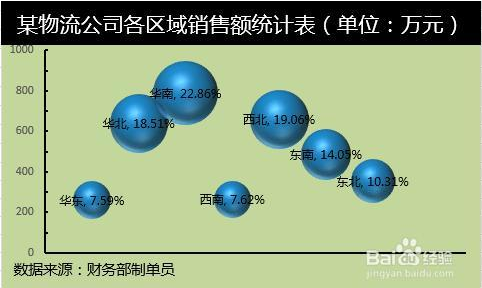
\includegraphics[scale=0.7]{li}
    			\caption{The 立体气泡图}
    			\label{fig:li}
    		\end{figure}
    	.\par	
    		18)热力图:热力图通过颜色不同展示不同的数据大小和分布情况
    		可以没有特定的自变量轴和因变量轴
    		经常与不同的背景(例如地图)结合\par
    		\begin{figure}[h!]
    			\centering
    			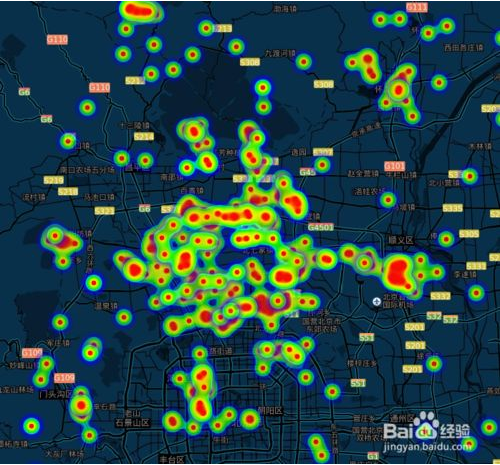
\includegraphics[scale=0.7]{re}
    			\caption{The 热力图}
    			\label{fig:re}
    		\end{figure}
    		19)矩形树图:适用于带有权重的层级数据(例如不同省份幼儿教师的学历比例情况)
    		通过小矩形面积的大小表示其在整体种的占比情况	\par
    		\begin{figure}[h!]
    			\centering
    			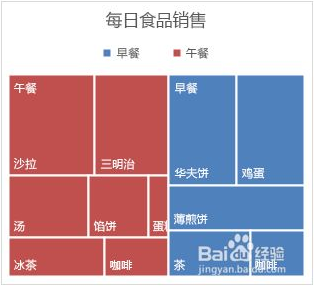
\includegraphics[scale=0.7]{ju}
    			\caption{The 矩形树图}
    			\label{fig:ju}
    		\end{figure}
    		20)弦图:数据分布在圆周的节点上
    		通过节点之间的连线来展示节点的关系
    		弦的两端宽度可以不相同,以展示权重关系\par
    		\begin{figure}[h!]
    			\centering
    			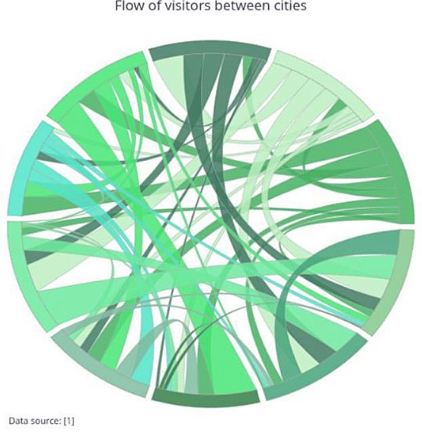
\includegraphics[scale=0.4]{xian}
    			\caption{The 弦图}
    			\label{fig:xian}
    		\end{figure}
    		21)桑吉图:一种描述多级数值流向的流程图
    		节点的不同长度代表了不同的数值大小
    		起始流量大小必须一致
    		不适宜展示带有权重的数值关系\par
    		\begin{figure}[h!]
    			\centering
    			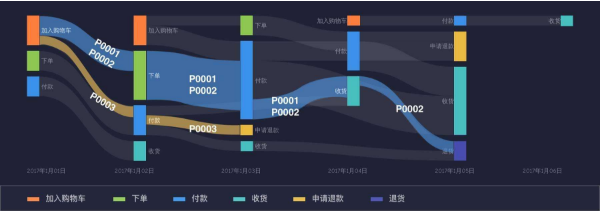
\includegraphics[scale=0.7]{sang}
    			\caption{The 桑吉图}
    			\label{fig:sang}
    		\end{figure}
    	e)可视化制作软件\par
    		1)Google Chart:Google Chart中有一大堆图表库,从线图到分层结构,可以满足任何需求。如果企业想深入挖掘,甚至可以寻求某种技术上的帮助。\par
    		2)D3:数据驱动的文档或D3是一个JavaScript库,可以为企业提供可视化大数据的任何方式。用户应该具备丰富的JavaScript知识来为收集的数据提供一个轮廓。被操纵的数据通过SVG、HTML和CSS来呈现,版本较旧的浏览器无法使用它。D3速度非常快,它支持实时数据集。\par
    		3)Highcharts:这是一个纯粹通过JavaScript创建的图表库,因此企业需要一点关于JavaScript的知识来实现??和使用这样一个工具。
    		Highcharts使用SVG、HTML5和VML,并通过不同的浏览器和iPhone和Android设备显示图表。这个工具需要2个.js文件用于任何特定的执行,这些文件通常在正常的网页上可用Highcharts可以足够有效地提供实时的JSON数据。\par
    		4)Datawrapper:Datawrapper是数据可视化工具之一,也得到了很快的发展,特别是那些利用它来设计图表和统计数据的媒体公司。这个工具有一个简单的导航过程,企业可以上传一个.csv文件来设计图表、地图、可视化等功能。\par
    		5)Jupyter:Jupyter被称为是大数据可视化的一站式商城,JupyteR是一个开源项目,通过十多种编程语言实现大数据分析、可视化和软件开发的实时协作。 它的界面包含代码输入窗口,并通过运行输入的代码以基于所选择的可视化技术提供视觉可读的图像。 Jupyter Notebook可以在团队中共享,以实现内部协作,并促进团队共同合作进行数据分析。 团队可以将Jupyter Notebook上传到GitHub或Gitlab,以便能共同合作影响结果。团队可以使用Kubernetes将Jupyter Notebook包含在Docker容器中,也可以在任何其他使用Jupyter的机器上运行Notebook。在最初使用Python和R时,JupyterNotebook正在积极地引入Java,Go,C#,Ruby等其他编程语言编码的内核。除此以外,Jupyter还能够与Spark这样的多框架进行交互,这使得对从具有不同输入源的程序收集的大量密集的数据进行数据处理时,Jupyte能够提供一个全能的解决方案。\par
    		6)Tableau:AI,大数据和机器学习应用可视化的最佳解决方案。Tableau可以与Amazon AWS,MySQL,Hadoop,Teradata和SAP协作,使之成为一个能够创建详细图形和展示直观数据的多功能工具。 这样高级管理人员和中间链管理人员能够基于包含大量信息且容易读懂的Tableau图形作出基础决策。\par
    	f)如何选择合适的可视化工具:\par
    	1.清晰、简洁和可定制的界面:\par   	
    	数据可视化程序的界面就像汽车仪表盘,你一眼就能得到想要的重要信息——从剩余油量、行车速度到续航里程。类似地,可视化界面应能在一个视图中显示所有关键信息。\par    	
    	一个好的数据可视化工具应该同时具备以下功能。首先样子看起来很酷。界面清晰又不失流行的颜色。太白令人厌烦,太多颜色感觉又乱,所以界面应该保持适当平衡。\par    	
    	其次,界面应该准确地展示所有重要的数据。比如用户关注的KPI、重要趋势或重要业务相关的数据集,都应该在界面一启动几秒钟内就能完整、清楚地显示出来。所有显示的内容应该一目了然。\par
    	界面还有一个非常重要的品质,是可定制化的。在不同时间段内,可能需要跟踪不同的数据集,那么需要自定义哪些数据重点显示。因此,数据可视化工具必须允许定制。\par    	
    	2.嵌入式\par	
    	要真正利用数据可视化的强大功能,将可视化报告无缝集成到其他应用程序中是非常重要的。为了让用户高效协同,跨平台共享报告,数据可视化软件应该兼容不同的应用程序。\par
    	并不是所有部门都需要分析所有数据。大多数人只希望数据的一部分与他们特定的应用程序无缝集成,从而帮助他们提高工作效率。所以一个好的数据可视化工具必须易于嵌入集成。\par
    	3.人机交互性\par
    	由数据可视化工具生成的可视化报告必须具有较强的人机交互性,支持调整一些变量或者参数,能够看到趋势/结果的随之变化。用户能够移动、排序、筛选相关变量,获得相应的效果。数据分析师和决策者需要的是,能够处理各种来源的数据并生成有价值内容的分析工具。可视化分析报告支持不同格式打开,可以在不同的时间突显不同的部分。\par
    	4.数据采集与共享\par   	
    	将原始数据导入可视化工具,然后以各种不同的形式导出可视化报告,这一过程要按照用户喜欢的方式进行。一些数据集可以最原始的形式输入到工具中,而另一些数据集则需要先进行聚合,因为它们太大了。有时,数据可以从一个数据源中获取,而有时需要从不同的数据源收集数据并通过工具进行可视化。有的数据可视化工具能从多个数据源收集数据并显示在同一个界面上,但有些工具可能没有此功能。您如何选择合适的工具就看具体的需求。需要自动化生成报告吗?团队之间是否需要共享分析报告?希望从报告中导出哪些数据呢?\par
    	5.地理标记和智能定位\par
    	如果您所处的领域对地理位置很关注,那么您可能需要地理和位置数据的可视化工具。比如这些数据来自哪里?哪些州或地区更积极?哪些领域需要拓展?对需要跟踪基于位置kpi的业务来说,按时间和空间分层数据集的能力非常重要。\par
    	6.数据挖掘\par
    	数据挖掘是研究大型数据集以识别其中的模式和趋势的过程。如果您处理大型数据集,并且希望可视化工具帮助提取其中的潜在信息并生成可视化报告,那么您需要可视化工具含有该功能。\par
    	7.人工智能\par
    	许多可视化工具在使用人工智能来分析、探索和预测趋势,并根据过去的变化预测未来的趋势。如果这是你感兴趣的东西,那么集成人工智能的可视化工具就非常适合。
\end{itemize}


\section{总结}
在这里,写自己对于整个课程和或本次报告的总结。\par
从开学到现在,在接触计算机的短短四个月中,就已经可以感受到计算机科学的美妙之处。在这个信息时代,人们和社会已经彻底离不开计算机了,计算机作为一项管理着全社会的信息科学产物,无时无刻都参与了我们的日常生活,人们用计算机对工作生活等进行着处理和规划,世界逐渐被串联在一起。\par


\section{附录}
\begin{itemize}
    \item  Github:https://github.com/BFXS/daolun
    		 \begin{figure}[h!]
    		\centering
    		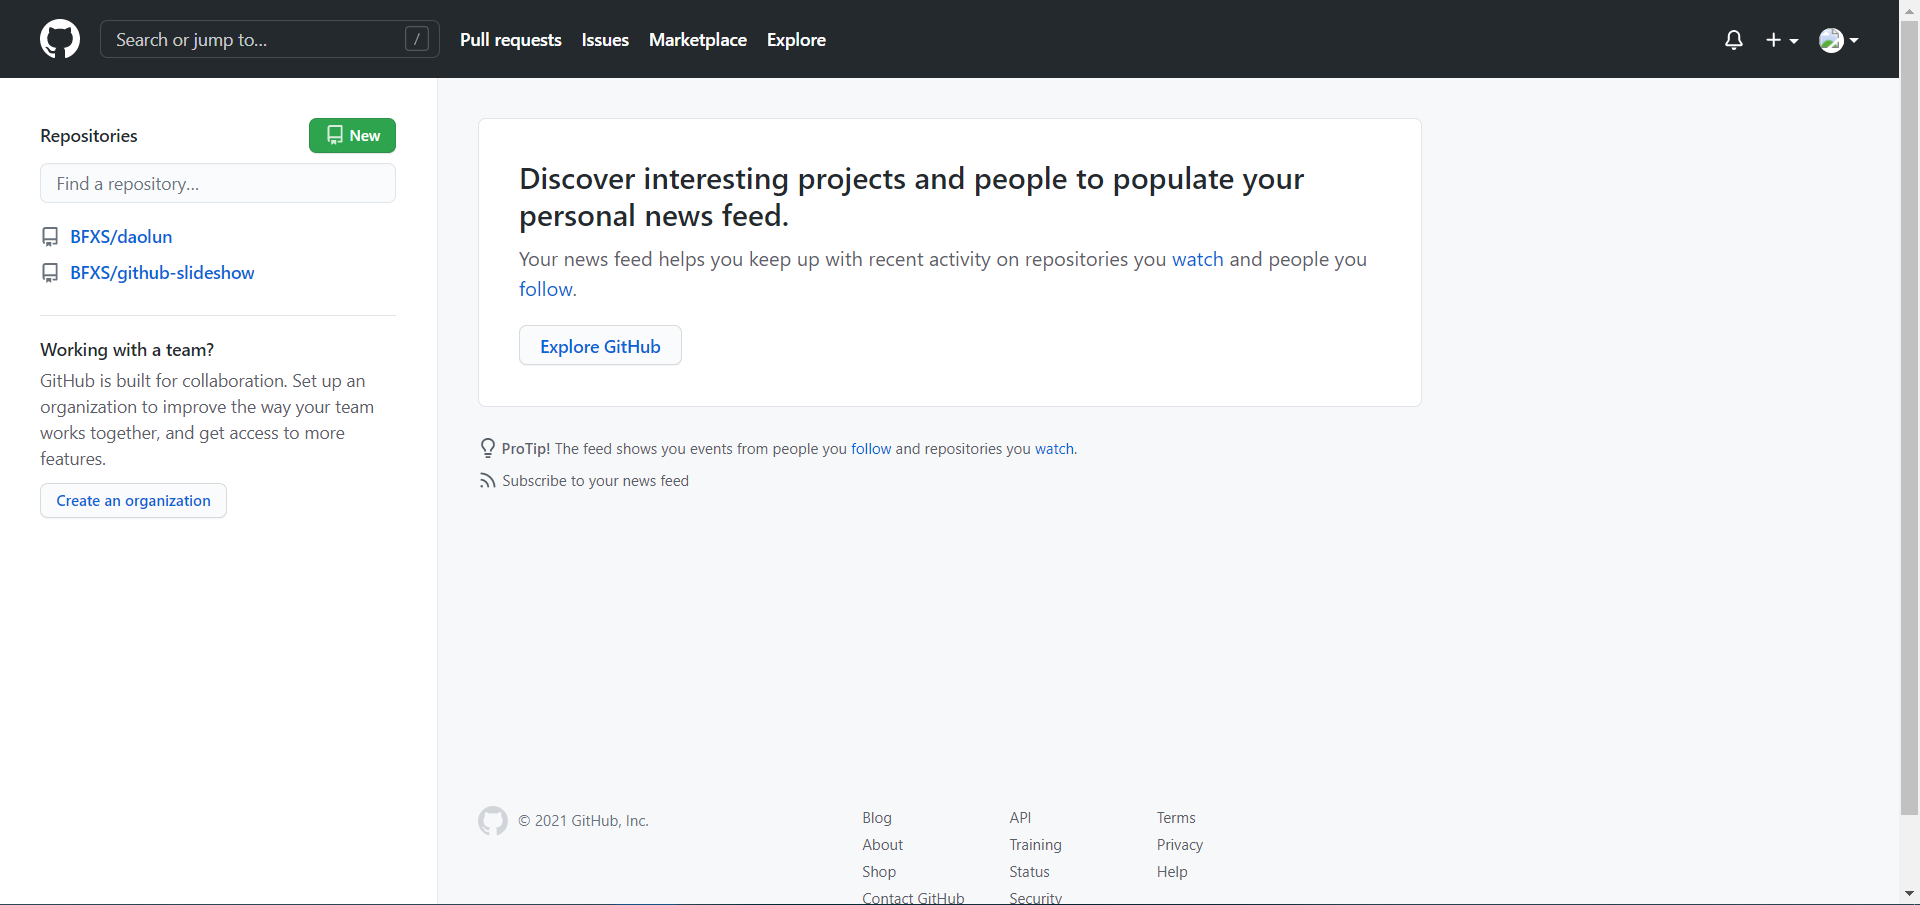
\includegraphics[scale=0.5]{github}
    		\caption{The Github截图}
    		\label{fig:github}
    		\end{figure}
    		观察者:
    		\begin{figure}[h!]
    			\centering
    			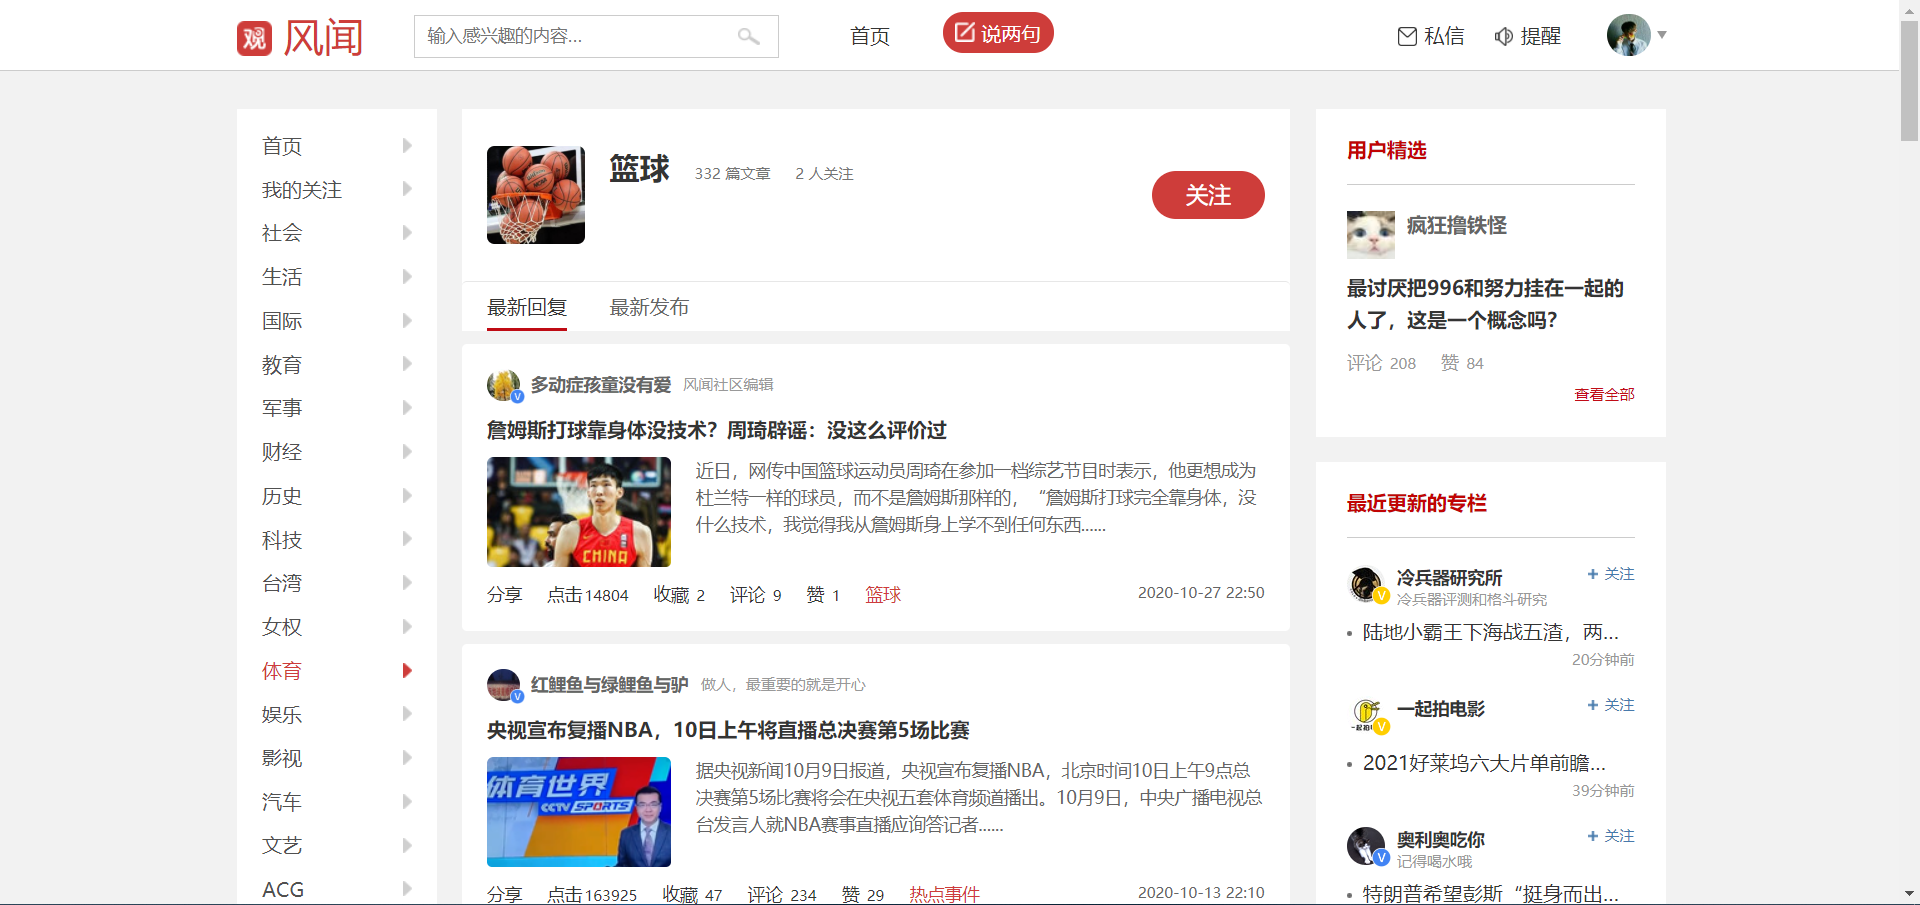
\includegraphics[scale=0.5]{guan1}
    			\caption{The 观察者网}
    			\label{fig:guan1}
    		\end{figure}
    	\begin{figure}[h!]
    		\centering
    		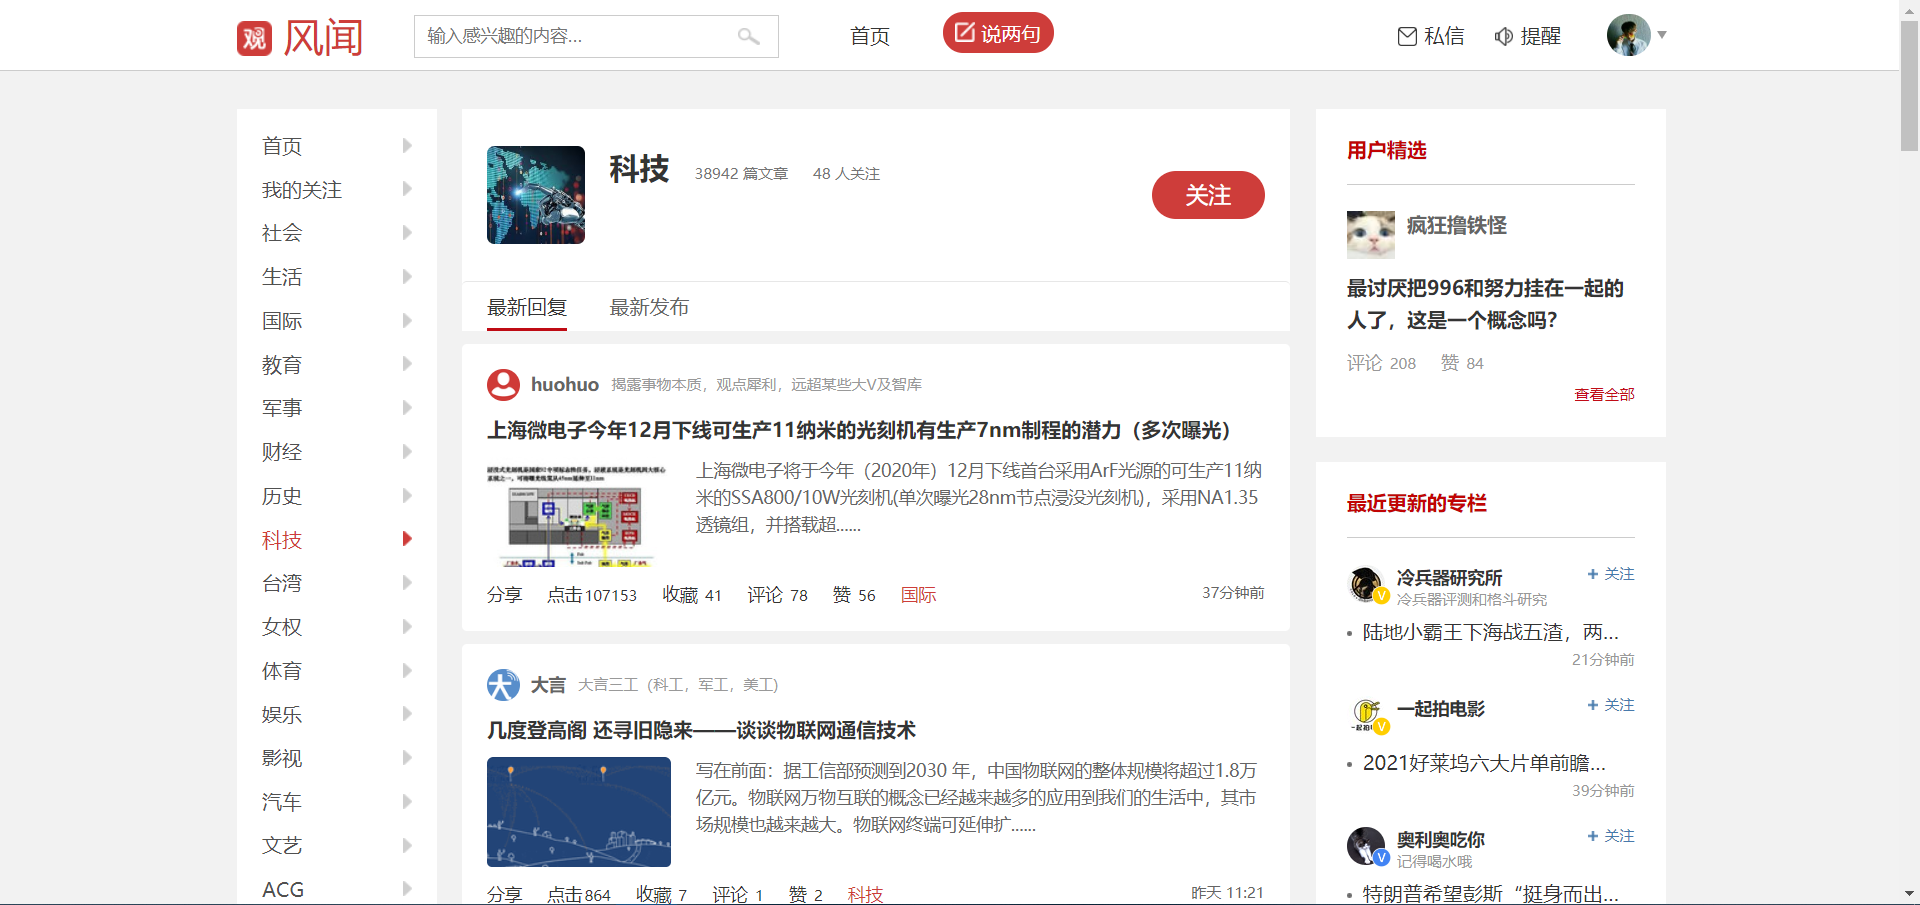
\includegraphics[scale=0.5]{guan2}
    		\caption{The 观察者网}
    		\label{fig:guan2}
    	\end{figure}
    		学习强国:
    		\begin{figure}[h!]
    		\centering
    		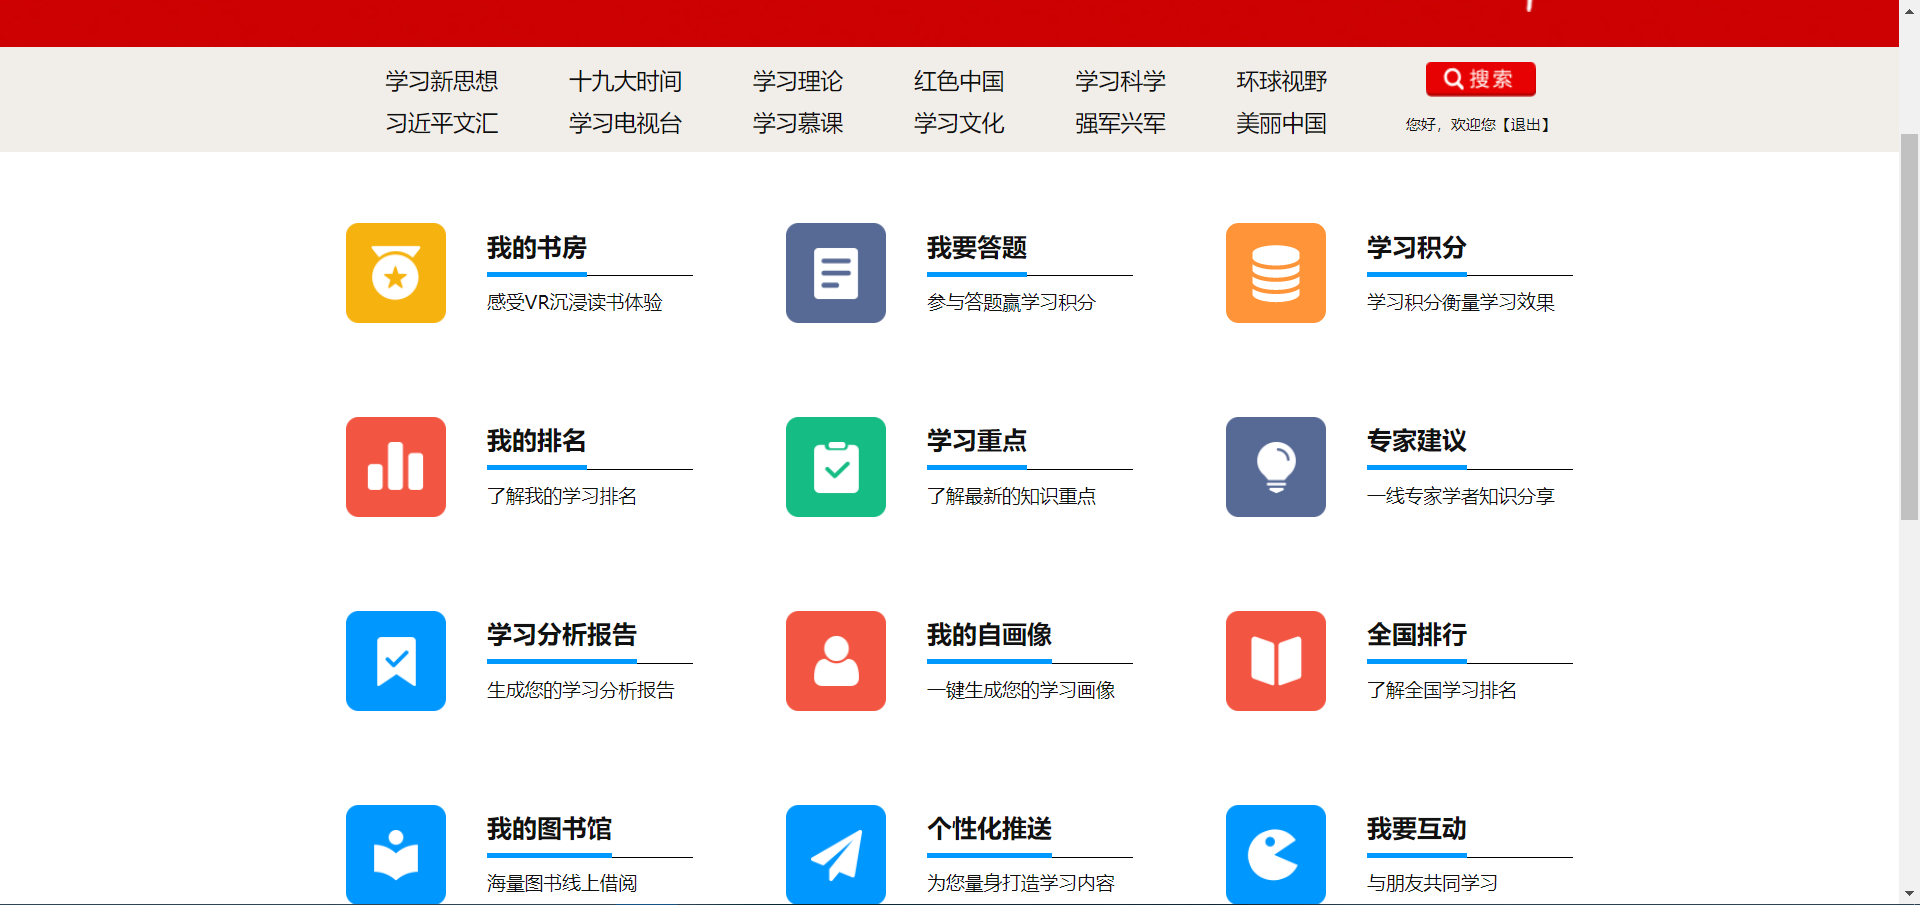
\includegraphics[scale=0.5]{xue}
    		\caption{The 学习强国}
    		\label{fig:xue}
    		\end{figure}
    		哔哩哔哩:
    		\begin{figure}[h!]
    			\centering
    			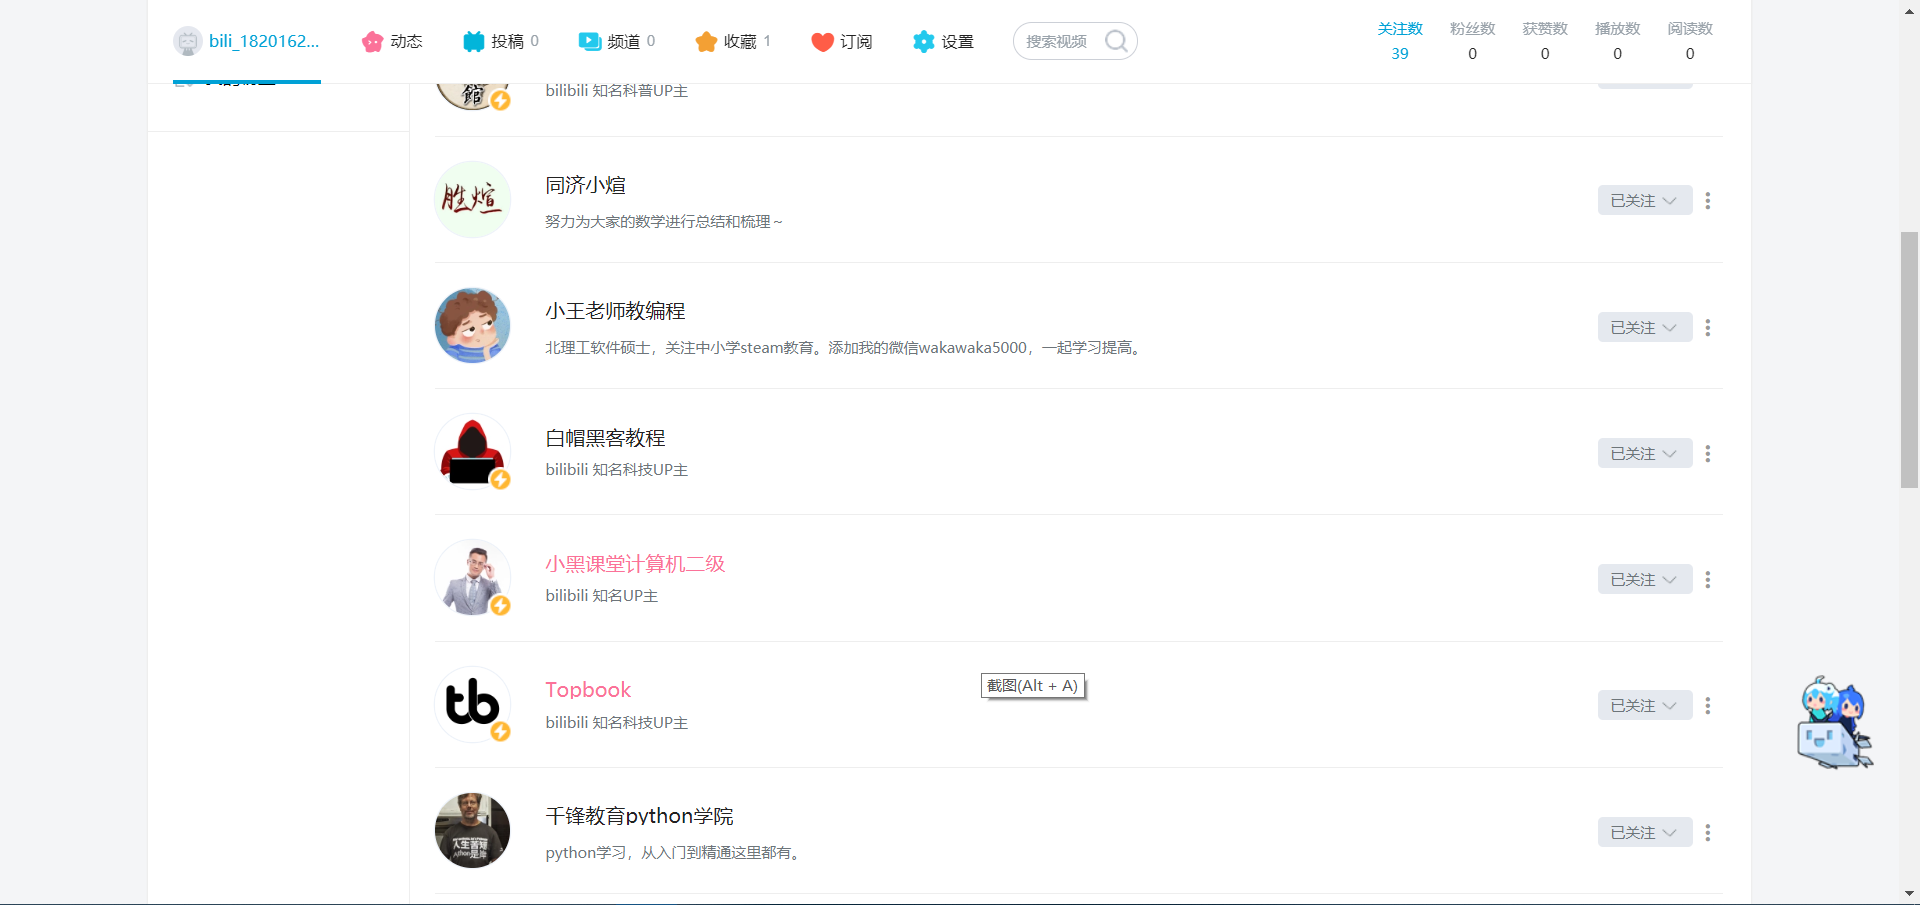
\includegraphics[scale=0.5]{b1}
    			\caption{The 哔哩哔哩}
    			\label{fig:b1}
    		\end{figure}
    	\begin{figure}[h!]
    		\centering
    		
\includegraphics[scale=0.5]{b2}
    		\caption{The 哔哩哔哩}
    		\label{fig:b2}
    	\end{figure}
    		CSDN(写的文章还有待更改,只是保存了文章,没有发布):\par
    		\begin{figure}[h!]
    			\centering
    			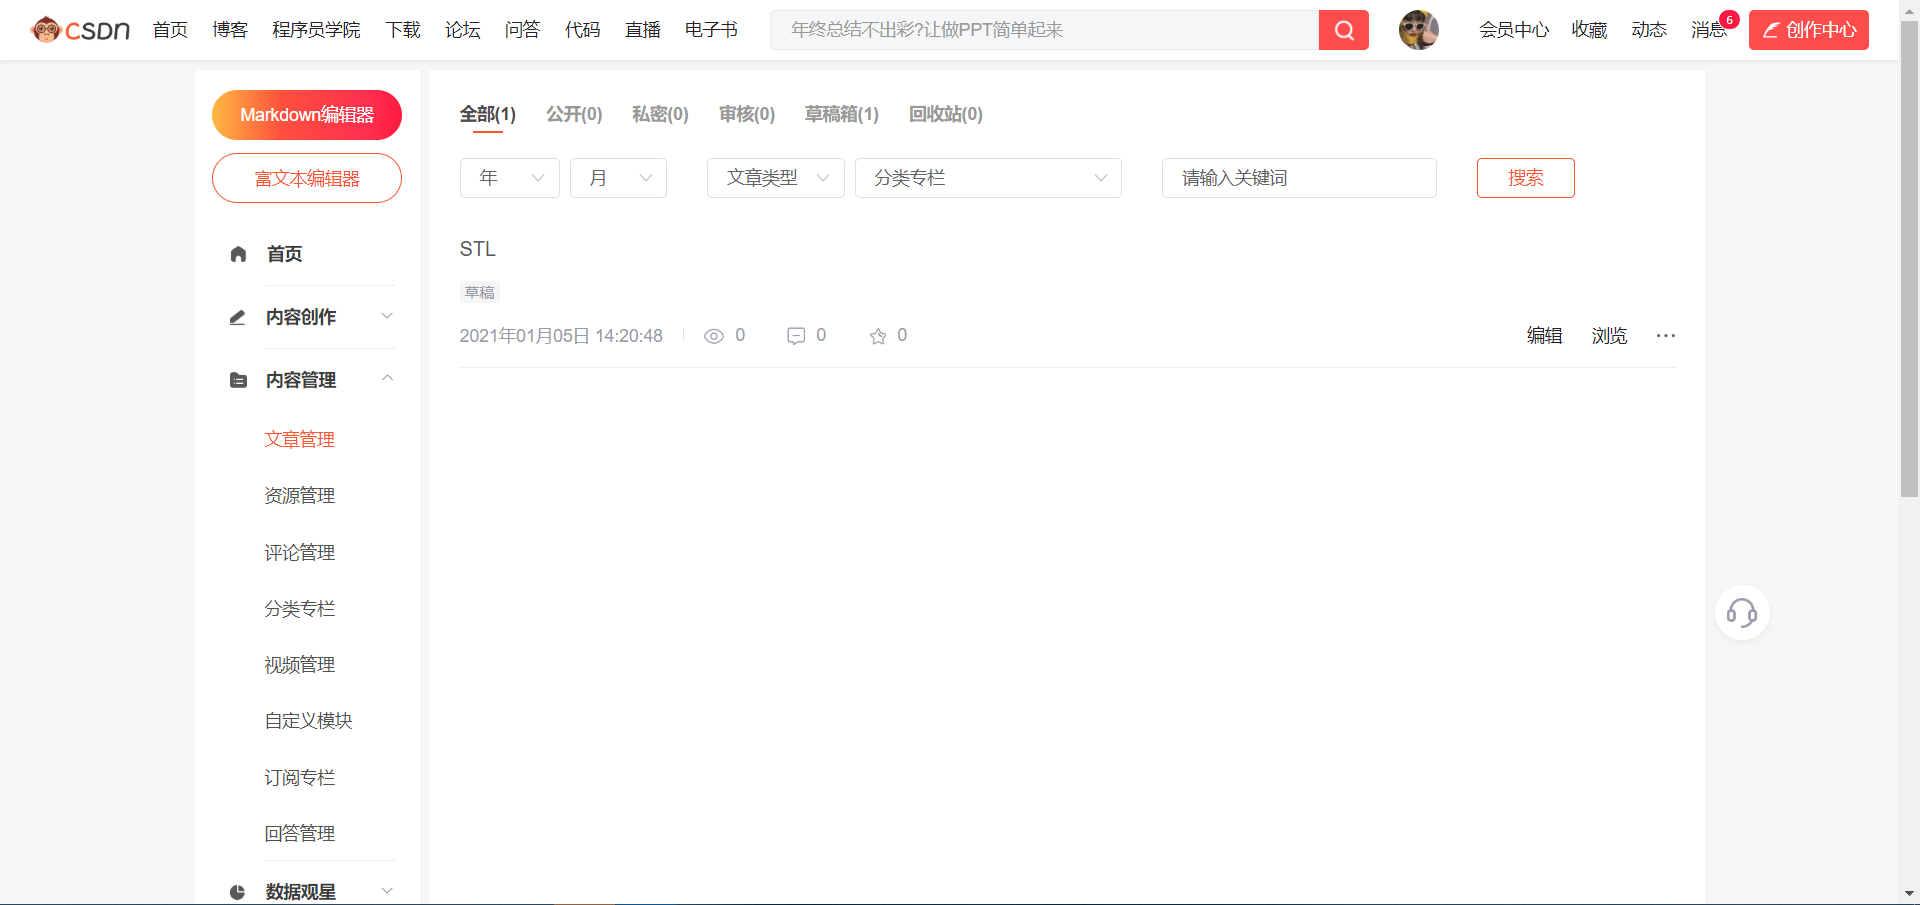
\includegraphics[scale=0.5]{CSDN}
    			\caption{The CSDN}
    			\label{fig:CSDN}
    		\end{figure}
    		博客园:
    		\begin{figure}[h!]
    			\centering
    			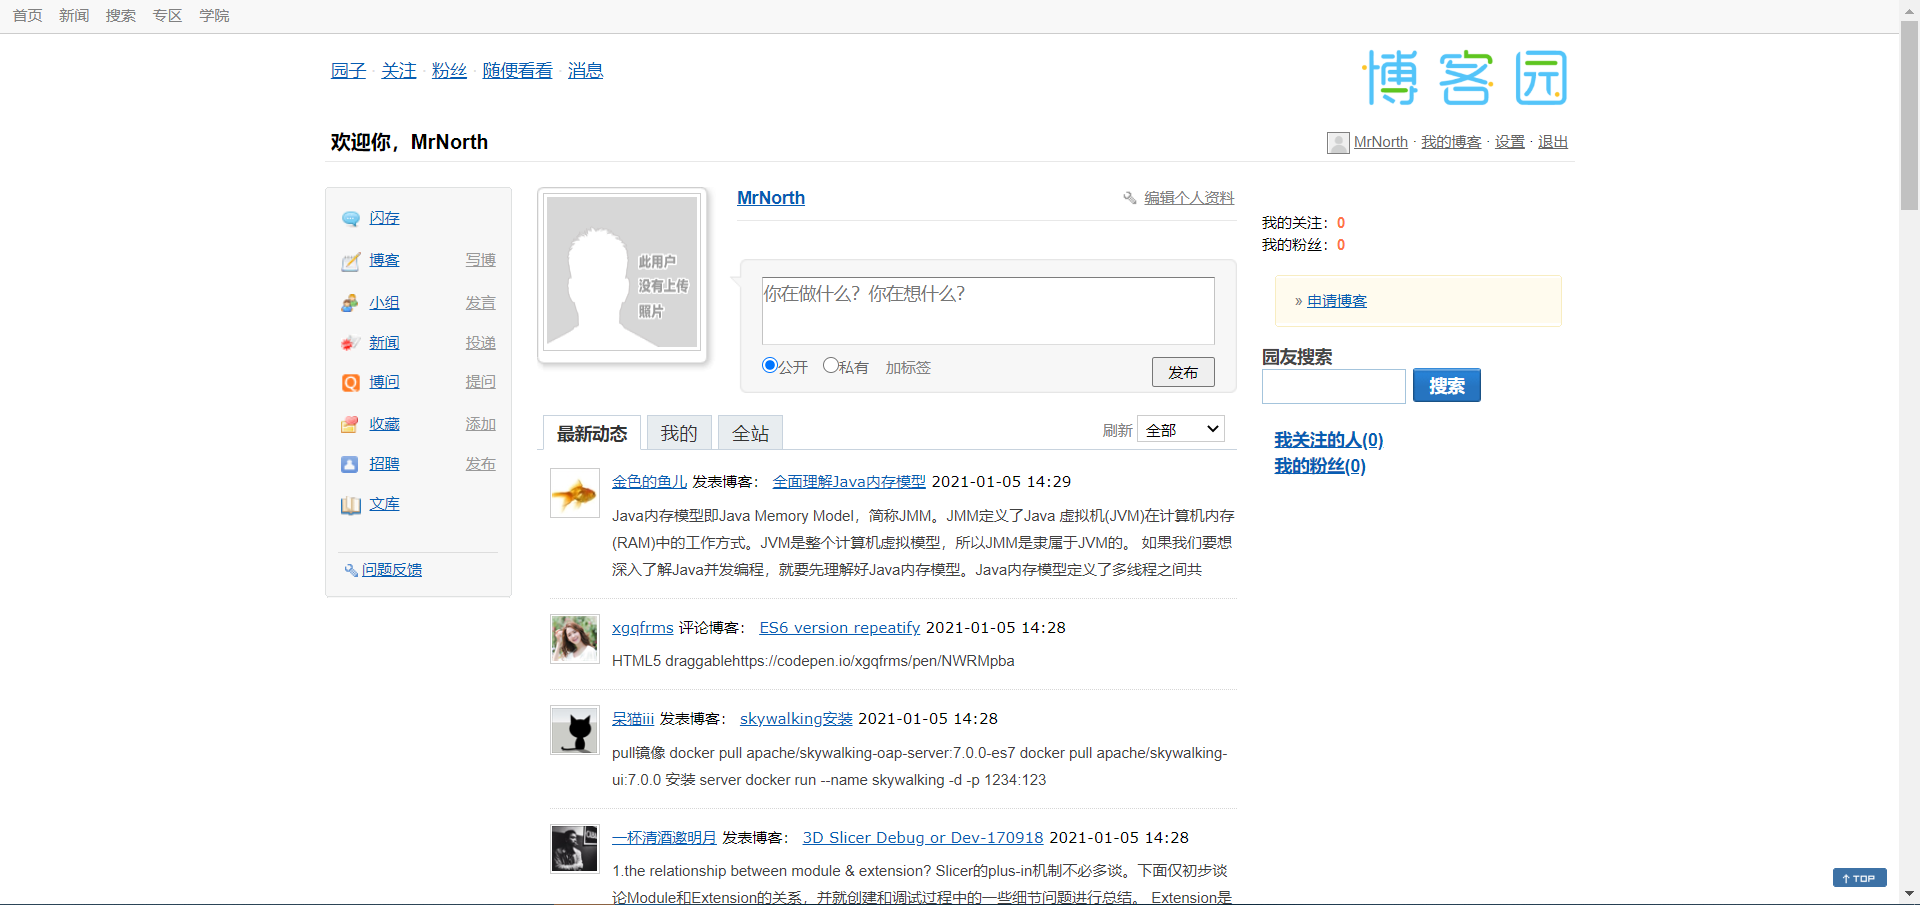
\includegraphics[scale=0.5]{bo}
    			\caption{The 博客园}
    			\label{fig:bo}
    		\end{figure}
    		
    .\par.\par.\par.\par
    

\end{itemize}

\hspace*{\fill} \\


\bibliographystyle{plain}
\bibliography{references}


\end{document}
